%%%%%%%%%%%%%%%%%%%%%%%%%%%%%%%%%%%%%%%%%%%%%%%%%%%%%%%%%%%%%%%%%%%%%%%%%%%%%%%%
%2345678901234567890123456789012345678901234567890123456789012345678901234567890
%        1         2         3         4         5         6         7         8

\documentclass[a4paper, 10 pt, conference]{ieeeconf} 
\usepackage{bbold}
\usepackage{xcolor}
\usepackage{hyperref}
\usepackage{graphicx}
\usepackage{booktabs}
\usepackage{colortbl}
\usepackage{ragged2e}
\usepackage{german}
%\selectlanguage{\german}
\selectlanguage{\english}
\usepackage{subfig}
%\usepackage[acronym]{glossaries}

%\usepackage{glossaries}

%\usepackage{biblatex}
%\{references.bib}

%\newacronym{GNN}{GNN}{global nearest-neighbour}
%\newacronym{RFS}{RFS}{Random Finite Sets}

%\define\gls{asd}

\def\andothers{\textit{et al.\,}}
\newcommand{\qq}[1]{{``#1''}}
\newcommand{\code}[1]{\textsf{#1}}

\overrideIEEEmargins                                      % Needed to meet printer requirements.

% See the \addtolength command later in the file to balance the column lengths
% on the last page of the document

% The following packages can be found on http:\\www.ctan.org
%\usepackage{graphics} % for pdf, bitmapped graphics files
%\usepackage{epsfig} % for postscript graphics files
%\usepackage{mathptmx} % assumes new font selection scheme installed
%\usepackage{times} % assumes new font selection scheme installed
%\usepackage{amsmath} % assumes amsmath package installed
%\usepackage{amssymb}  % assumes amsmath package installed

\title{\LARGE \bf
  From Enterprise Models to Dimensional Models: A Tool to transform your database \\
  Data Modelling Course Project
}


\author{
Jonas Munch {\tt\small j.munch@campus.fct.unl.pt} \\
Dusan Zeliar {\tt\small d.zeliar@campus.fct.unl.pt}
}

\begin{document}

\maketitle
\thispagestyle{empty}
\pagestyle{empty}

% TODO list:
% - Note density form of p(OperatorScore | TrackClass)


%%%%%%%%%%%%%%%%%%%%%%%%%%%%%%%%%%%%%%%%%%%%%%%%%%%%%%%%%%%%%%%%%%%%%%%%%%%%%%%%
\begin{abstract}
This technical report describes our work of the Data Modelling class 2017.
The goal of this work is to implement a tool that supports the user to transform a relational schemed database (OLTP) into a dimensional model (OLAP).
Based on an approach proposed by Moody %TODO ref
a so called star schema will be produced out of an arbitrary database.

The program guides the user via commandline interface through all the neccessary steps to find an agreement of which tables are selected as transaction entities, component entities and classification entities.

% TODO eventually add Aggregation operator

As soon as the selection phase is done, our software will generate a dimensional model based on the input scheme and populate it from the original data.

\end{abstract}


%%%%%%%%%%%%%%%%%%%%%%%%%%%%%%%%%%%%%%%%%%%%%%%%%%%%%%%%%%%%%%%%%%%%%%%%%%%%%%%%
\section{Introduction}
\label{sec:introduction}
In recent years the increasing amount


\section{Theory}
\label{sec:theory}
%State of the art

The method for developing dimensional models from Entity Relationship models proposed by Moody \andothers in \cite{moody2000enterprise} was used by us as a basis to implement the program.
The method is here only quicly outlined, for deeper information refer to the original paper.
Moody's method consists basically of three steps:

\paragraph{Classify Entities}
\label{par:classifyEntities}

In the first step the entities of the Entity Relationship model need to be classified into one of the following categories: \emph{transaction}, \emph{component} or \emph{classification}.

The transaction tables describe certain events that occur in the business (\eg sales in a retail store) and contain measurements or quantities that my be summarized.
The transaction tables are the most important in a data warehouse and will result later in so called \emph{fact tables}.

A component entity contains further information about the facts in the transaction tables and will therefore result later in so called \emph{dimension tables} of a star schema.
The components are directly related to the transaction entities via a one-to-many relationship.

Other tables that are related, directly or transitively, to the component via one-to-many relationships will be categorized as classification entities.
They are adding even more information (can be more abstract or more detailed) to the components and will accordingly end up in the dimension tables.

\paragraph{Identify Hierarchies}

\emph{Hierarchies} in terms of \cite{moody2000enterprise} are chains of one-to-many relationships, all aligned in the same direction.
The terms \emph{minimal} and \emph{maximal} are introduced in this context.
Entities are called minimal if they occur at the bottom of a hierarchy chain, and are called maximal if they occur at the top.
Hierarchies are important, because they can be collapsed.
Collapsing is an important step in simplifying the database schema by introducing redundancy.

\paragraph{Produce Dimensional Models}

In  order to transform the database, Moody describes two operators.
Firstly the hierarchies found in the step before get \emph{collapsed}.
Beginning at the maximal entities the data is gradually merged into the entity's child table: By resolving foreign key constraints the data is duplicated and redundancy is produced.
This process can be continued until the minimal entity is reached and all the data is located in a single table.
However, for generating a star schema the collapsing process should be stopped when a component entity is reached in order to construct a proper dimension.

The second operator is called \emph{aggregation} and can be applied optionally.
The goal here is to summarize the data in order to present it in a more compressed way (by doing this we will lose detail of information that cannot be reversed).
To achieve aggregation, columns of a table must be selected to act as aggregation keys (by which the data will be grouped) and an aggregation function must be specified for the aggregated columns (numerical attributes like price, quantity, etc.).



\section{Implementation}
\label{sec:implementation}
\subsection{Application Design}

The tool we implemented is designed as pipeline that takes an arbitrary database as input and outputs a set of SQL scripts, which can be run to create a new database having a dimensional scheme.
The user is guided throughout the whole process via a command line interface, which enforces him to do the steps in the right order.
As a special feature we implemented a mechanism to save the current working state in order to continue the work at a later point in time.
As soon as all the specifications about the resulting scheme are made, the program will output and run the resulting SQL scripts in a way that the new database is created and the original data is populated.

\paragraph{Making suggestions}

The program tries to support the user in a helpful way.
After the input database scheme is read, the system will come up with some suggestions for the categorization of tables (according to \ref{par:classifyEntities}) into \emph{transaction}, \emph{component} and \emph{classification}.

Since it is a hard job to find transaction candidates from only the database schema without knowing about the business, we decided to use a different approach.
It is likely that the user will choose a minimal entity as transaction because it is one of the roots of the database and therefore a very important table for the business.
In order to obtain every minimal entity we find every table that is not referenced by any foreign key.
As we consider the database scheme as a directed graph (tables are nodes and foreign keys are directed edges) we can speak about the transaction tables as roots of a spanning tree.
The direct neighbours of the roots are suggested to be classified as components.
Every other table that is part of the spanning tree, \ie reachable by foreign keys from the root, is suggested to be a classification table.

For sure, if the user not satisfied with this suggestion he can alter the classification at the given time to fulfill his needs.

\paragraph{User interaction}

The generation of a dimensional model cannot be done completely automatically.
The user's needs and desires are unpredictable and the according structure of dimensional model as well.
Therefore we need user interaction letting him input his needs as well as supervision and confirmation throughout the process.
In order to accomplish that, we implemented a commandline interface which guides the user step by step helping him to give the commands in the right order.
Every time a suggestion is made, it is presented to the user, letting him modify for his special needs and confirm when he thinks the right design is chosen.
Since we aware that mistakes can happen, the program offers an undo-option at certain points in the process.

At very first, the input database scheme is parsed and displayed to the user to give a overview of what to do. Figure~\ref{fig:metadataOutput} shows a short version of this output.
After the database scheme is parsed, a suggestion of transaction tables is made.
See in figure~\ref{fig:transactionSuggestion} how the suggestion is presented to the user.
The transaction entities form the core of the dimensional model because they will result into fact tables.
That is why the user must select the transaction entities prior to any other step.

When the transaction entities are selected the system can proceed to suggest component and classification entities.
Figure~\ref{fig:dimensionalModelSuggestion} shows the interface of this step. Here the user can also classify some table as \emph{unclassified} which basically means, that the table's columns and data will not occur in the resulting dimensional scheme.

The information collected by now is sufficient to create a dimensional scheme.
Moody \andothers propose in \cite{moody2000enterprise} a second optional step, the \emph{aggregation}.
Hence the user is given the ability now to choose columns from every transaction table to be aggregated.
Doing this he also needs to specify an aggregation function.

Are all this steps completed, the program will generate the necessary SQL scripts and run them automatically.

However, we know that using the program is hard work including many steps, so the user may want to have a coffee when the work is halfway done.
Being aware of this the program comes with a handy feature to save the current working state at any time.
The work done so far can be saved as a JSON-file and loaded into the program again to continue working from that point.

\paragraph{Generating SQL}

The generating process starts by forming a graph-like structure of entities.
Independent structures are created for each of the transaction and component entities, which are set as the roots.
Using depth first search approach, all of the referenced entities from root are processed.
Processing of entities consists of creating parts of the final SQL query.
Depending of entity type and its position in graph, different SQL query parts are created.
By aggregating data from all structures, final SQL queries for creating new table and migrating data are made.
\par
Process of aggregating columns data in transaction tables consists of defining data types of aggregated columns, setting columns names and generating migrating SQL scripts.  

\subsection{Implementation Details}

\begin{figure}
  \centering
  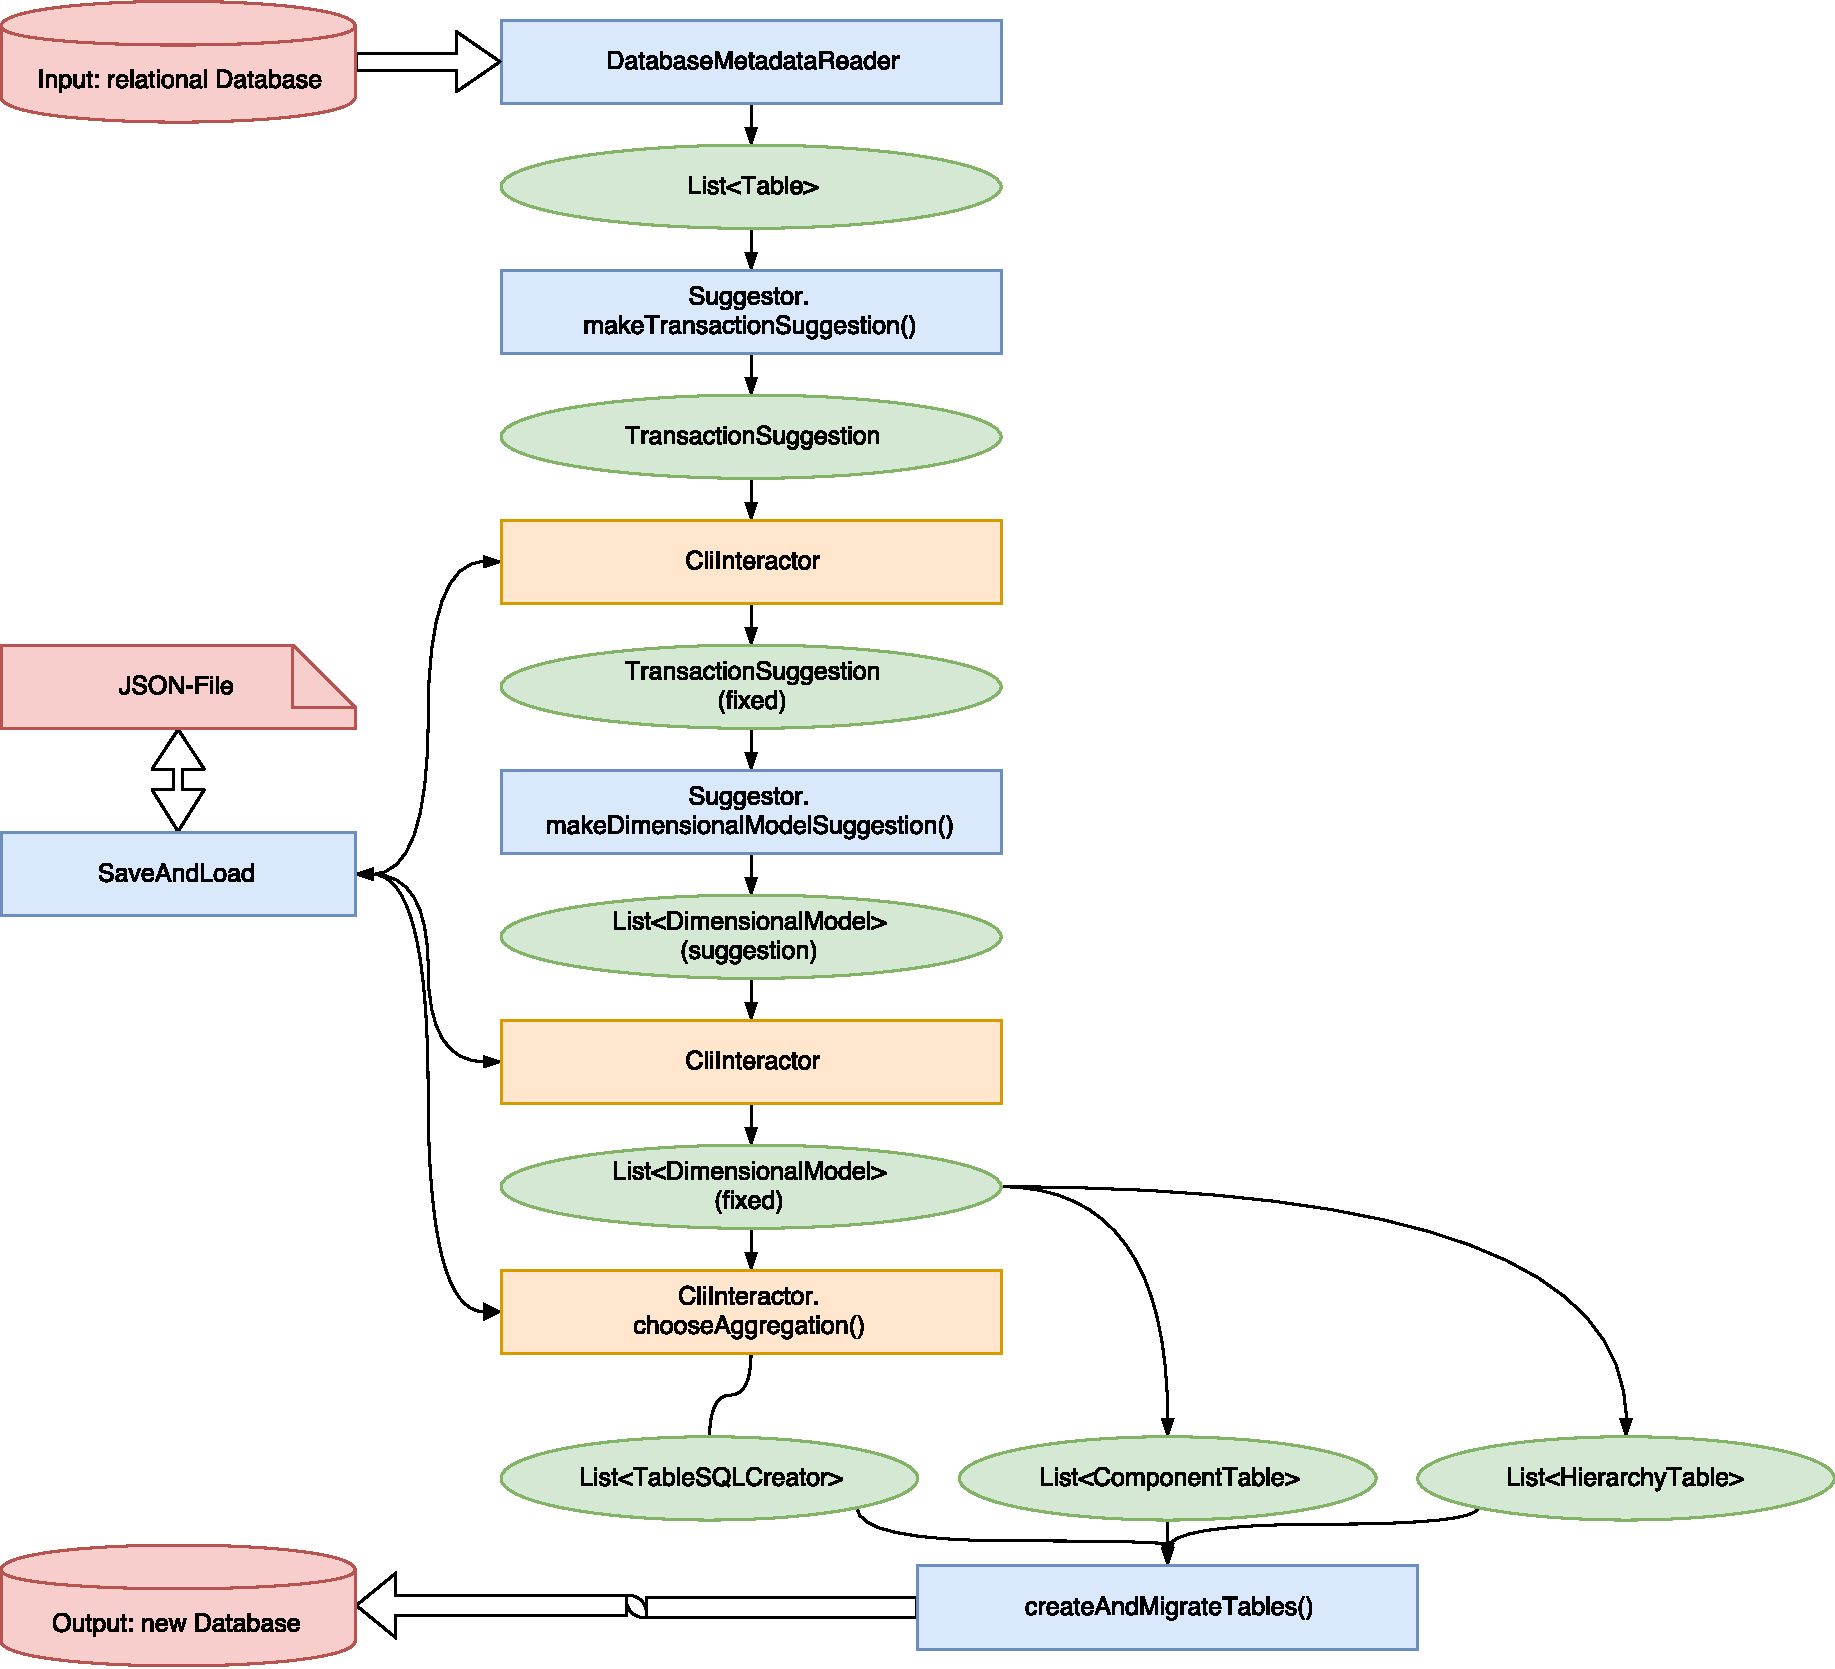
\includegraphics[width=\linewidth]{images/dataFlowDiagram}
  \caption{Dataflow Diagram of the Pipeline.}
  \label{fig:dataflowDiagram}
\end{figure}

As a first step the input database is parsed using the JDBC library\footnote{\url{http://www.oracle.com/technetwork/java/javase/jdbc/index.html}}.

JDBC is also used to retrieve information about foreign key constraints: The transaction table suggestions, which are based on the number of referencing tables, are made by using this information.

With list of all tables in source database, \texttt{TransactionSuggestion} creates default suggestion of classification of entities based on number of foreigh keys referencing each table.
Suggestion is presented to user by \texttt{TransactionSuggestion} class which also handles following user modification of final tables classification.

The main algorithm of collapsing multiple tables to one is implemented in class \texttt{HierarchyTable} and its method \texttt{createReferencedTableList(List<Table> allTabs)}.

Starting from root table, this function is recursive called on all of the referred tables. To every lower level of graph, a table prefix is distributed to keep track of actual table level and its path from root.
In case of multiple keys referring one table, foreigh key is taken into account. After all refered tables are processed, actual table creates its own parts of SQL query.
The root table then creates final sql query with \texttt{createFinalSqlScripts()}, which extracts query parts of all tables and put it into final queries.
Migration is handled by \texttt{createAndMigrateTable(Credentials credentials, String select, String insert, String create)} by running create, select and in sert query creating a new record for all retrieved source data.

\begin{figure}[p]
  \lstinputlisting[breaklines]{images/createReferencedTable.txt}
  \caption{Process intity structure}
  \label{fig:metadataOutput}
\end{figure}

\begin{figure}[p]
  \lstinputlisting[breaklines]{images/metadataOutput.txt}
  \caption{Output of parsed metadata}
  \label{fig:metadataOutput}
\end{figure}

\subsection{Usage of the Tool}

Usage consists of three steps.
First step lists first suggestion of tables classification and allows to change transaction entities.
Seconds step allows to filter component and classification tables, which will be migrated.
Finally, a form of star schema is specified, either one connected star schema, or own star for each transaction entity.

\begin{figure}[p]
  \lstinputlisting[breaklines]{images/transactionSuggestion.txt}
  \caption{Commandline interface: Suggestion and Selection of \emph{Transaction entities}}
  \label{fig:transactionSuggestion}
\end{figure}

\begin{figure}[p]
  \lstinputlisting[breaklines]{images/dimensionalModelSuggestion.txt}
  \caption{Commandline interface: Suggestion and Selection of \emph{Component and Classification entities}}
  \label{fig:dimensionalModelSuggestion}
\end{figure}

\begin{figure}[p]
  \lstinputlisting[breaklines]{images/aggregationSelection.txt}
  \caption{Commandline interface: Selection of \emph{Aggregation functions}}
  \label{fig:aggregationSelection}
\end{figure}



\section{Evaluation}
\label{sec:evaluation}
The evaluation was perfomed by recreating example OLAP database from moody.
We created copy of OLTP database and run application with the same entities classification.
A new star schema database was created and the data were successfully migrated.
\begin{figure}
  \centering
  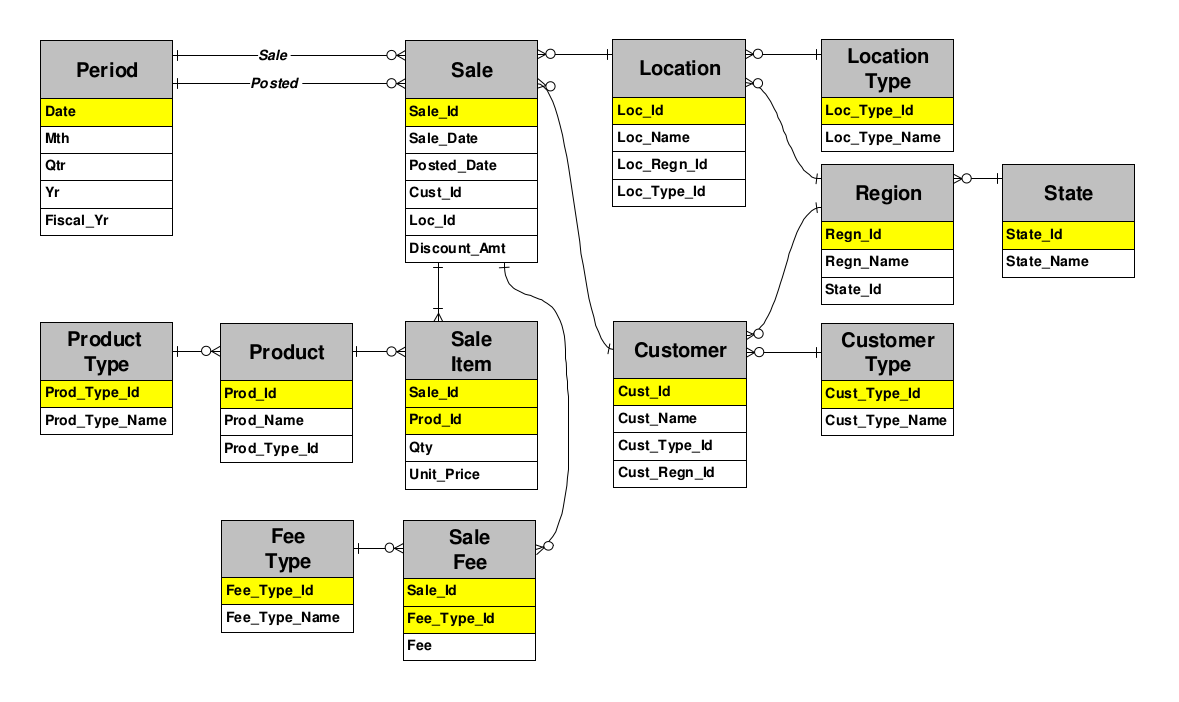
\includegraphics[width=\linewidth]{images/exampleDatabase}
  \caption{Example OLTP database scheme by Moody \andothers \cite{moody2000enterprise}}
  \label{fig:exampleDatabase}
\end{figure}

\begin{figure}
  \centering
  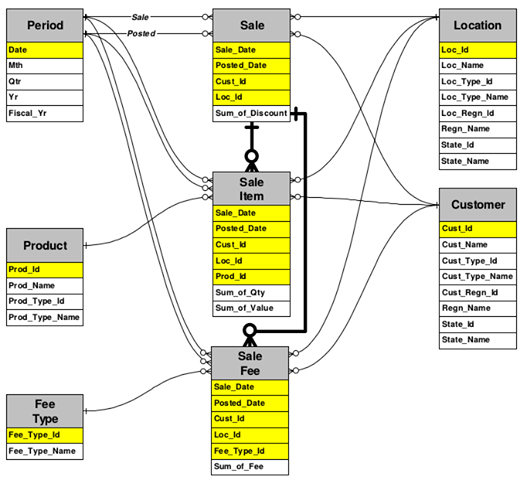
\includegraphics[width=\linewidth]{images/exampleDatabaseStarModel}
  \caption{Created example OLAP database scheme by Moody \andothers \cite{moody2000enterprise}}
  \label{fig:exampleDatabaseStarModel}
\end{figure}


\section{Conclusion}
\label{sec:conclusion}
In this project, we implemented and tested creation of a basic dimensional model from Entity Relationship model. After studying existing methods of creating dimensional models we proposed an application. The application work flow starts with getting source database schema, suggesting a classification of entities and identifying hierarchies in model. The next step is collapsing hierarchies and aggregating data. Finally a new dimensional model database is created and the data is migrated. 	The created dimensional database is in a form of a star schemas, each start consists of a fact table and its dimensions. The schema shares the same dimensions between fact tables but does not contain connection between fact tables.
	The developed application can be extended by a connection between facts table to contain full star scheme of source database.
  


\section{How to use Latex}
% TODO remove this section
\subsection{Example Section}

Lorem ipsum dolor sit amet, consetetur sadipscing elitr, sed diam nonumy eirmod tempor invidunt ut labore et dolore magna aliquyam erat, sed diam voluptua. At vero eos et accusam et justo duo dolores et ea rebum. Stet clita kasd gubergren, no sea takimata sanctus est Lorem ipsum dolor sit amet. Lorem ipsum dolor sit amet, consetetur sadipscing elitr, sed diam nonumy eirmod tempor invidunt ut labore et dolore magna aliquyam erat, sed diam voluptua. At vero eos et accusam et justo duo dolores et ea rebum. Stet clita kasd gubergren, no sea takimata sanctus est Lorem ipsum dolor sit amet. Lorem ipsum dolor sit amet, consetetur sadipscing elitr, sed diam nonumy eirmod tempor invidunt ut labore et dolore magna aliquyam erat, sed diam voluptua. At vero eos et accusam et justo duo dolores et ea rebum. Stet clita kasd gubergren, no sea takimata sanctus est Lorem ipsum dolor sit amet.   

Duis autem vel eum iriure dolor in hendrerit in vulputate velit esse molestie consequat, vel illum dolore eu feugiat nulla facilisis at vero eros et accumsan et iusto odio dignissim qui blandit praesent luptatum zzril delenit augue duis dolore te feugait nulla facilisi. Lorem ipsum dolor sit amet, consectetuer adipiscing elit, sed diam nonummy nibh euismod tincidunt ut laoreet dolore magna aliquam erat volutpat.   

Ut wisi enim ad minim veniam, quis nostrud exerci tation ullamcorper suscipit lobortis nisl ut aliquip ex ea commodo consequat. Duis autem vel eum iriure dolor in hendrerit in vulputate velit esse molestie consequat, vel illum dolore eu feugiat nulla facilisis at vero eros et accumsan et iusto odio dignissim qui blandit praesent luptatum zzril delenit augue duis dolore te feugait nulla facilisi.   

Klassifikation von Mustern wurde beschrieben in \cite{Niemann2007KVM}

\paragraph{Figures}

\begin{figure}[tb]
  \centering
  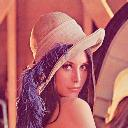
\includegraphics[width=0.8\linewidth]{images/lena}
  \caption{Lena}\label{f:lena}
\end{figure}

Jedes Bild sollte auch im Text erwähnt werden, so z.\,B.\ \figurename~\ref{f:lena}.

\paragraph{Formulas}

\[
  f(x) = \sum_{i=0}^N a_i \cdot h(x)
\]

Und auch in Fließtext $f(x) = \sum_{i=0}^N a_i \cdot h(x)$.


\addtolength{\textheight}{0cm}   % This command serves to balance the column lengths
                                  % on the last page of the document manually. It shortens
                                  % the textheight of the last page by a suitable amount.
                                  % This command does not take effect until the next page
                                  % so it should come on the page before the last. Make
                                  % sure that you do not shorten the textheight too much.

%%%%%%%%%%%%%%%%%%%%%%%%%%%%%%%%%%%%%%%%%%%%%%%%%%%%%%%%%%%%%%%%%%%%%%%%%%%%%%%%



%%%%%%%%%%%%%%%%%%%%%%%%%%%%%%%%%%%%%%%%%%%%%%%%%%%%%%%%%%%%%%%%%%%%%%%%%%%%%%%%



%%%%%%%%%%%%%%%%%%%%%%%%%%%%%%%%%%%%%%%%%%%%%%%%%%%%%%%%%%%%%%%%%%%%%%%%%%%%%%%%
\section*{Acknowledgment}


%%%%%%%%%%%%%%%%%%%%%%%%%%%%%%%%%%%%%%%%%%%%%%%%%%%%%%%%%%%%%%%%%%%%%%%%%%%%%%%%

\bibliographystyle{plain}
\bibliography{references}

\end{document}
